% Options for packages loaded elsewhere
\PassOptionsToPackage{unicode}{hyperref}
\PassOptionsToPackage{hyphens}{url}
%
\documentclass[
]{article}
\usepackage{lmodern}
\usepackage{amssymb,amsmath}
\usepackage{ifxetex,ifluatex}
\ifnum 0\ifxetex 1\fi\ifluatex 1\fi=0 % if pdftex
  \usepackage[T1]{fontenc}
  \usepackage[utf8]{inputenc}
  \usepackage{textcomp} % provide euro and other symbols
\else % if luatex or xetex
  \usepackage{unicode-math}
  \defaultfontfeatures{Scale=MatchLowercase}
  \defaultfontfeatures[\rmfamily]{Ligatures=TeX,Scale=1}
\fi
% Use upquote if available, for straight quotes in verbatim environments
\IfFileExists{upquote.sty}{\usepackage{upquote}}{}
\IfFileExists{microtype.sty}{% use microtype if available
  \usepackage[]{microtype}
  \UseMicrotypeSet[protrusion]{basicmath} % disable protrusion for tt fonts
}{}
\makeatletter
\@ifundefined{KOMAClassName}{% if non-KOMA class
  \IfFileExists{parskip.sty}{%
    \usepackage{parskip}
  }{% else
    \setlength{\parindent}{0pt}
    \setlength{\parskip}{6pt plus 2pt minus 1pt}}
}{% if KOMA class
  \KOMAoptions{parskip=half}}
\makeatother
\usepackage{xcolor}
\IfFileExists{xurl.sty}{\usepackage{xurl}}{} % add URL line breaks if available
\IfFileExists{bookmark.sty}{\usepackage{bookmark}}{\usepackage{hyperref}}
\hypersetup{
  hidelinks,
  pdfcreator={LaTeX via pandoc}}
\urlstyle{same} % disable monospaced font for URLs
\usepackage[margin=1in]{geometry}
\usepackage{color}
\usepackage{fancyvrb}
\newcommand{\VerbBar}{|}
\newcommand{\VERB}{\Verb[commandchars=\\\{\}]}
\DefineVerbatimEnvironment{Highlighting}{Verbatim}{commandchars=\\\{\}}
% Add ',fontsize=\small' for more characters per line
\usepackage{framed}
\definecolor{shadecolor}{RGB}{248,248,248}
\newenvironment{Shaded}{\begin{snugshade}}{\end{snugshade}}
\newcommand{\AlertTok}[1]{\textcolor[rgb]{0.94,0.16,0.16}{#1}}
\newcommand{\AnnotationTok}[1]{\textcolor[rgb]{0.56,0.35,0.01}{\textbf{\textit{#1}}}}
\newcommand{\AttributeTok}[1]{\textcolor[rgb]{0.77,0.63,0.00}{#1}}
\newcommand{\BaseNTok}[1]{\textcolor[rgb]{0.00,0.00,0.81}{#1}}
\newcommand{\BuiltInTok}[1]{#1}
\newcommand{\CharTok}[1]{\textcolor[rgb]{0.31,0.60,0.02}{#1}}
\newcommand{\CommentTok}[1]{\textcolor[rgb]{0.56,0.35,0.01}{\textit{#1}}}
\newcommand{\CommentVarTok}[1]{\textcolor[rgb]{0.56,0.35,0.01}{\textbf{\textit{#1}}}}
\newcommand{\ConstantTok}[1]{\textcolor[rgb]{0.00,0.00,0.00}{#1}}
\newcommand{\ControlFlowTok}[1]{\textcolor[rgb]{0.13,0.29,0.53}{\textbf{#1}}}
\newcommand{\DataTypeTok}[1]{\textcolor[rgb]{0.13,0.29,0.53}{#1}}
\newcommand{\DecValTok}[1]{\textcolor[rgb]{0.00,0.00,0.81}{#1}}
\newcommand{\DocumentationTok}[1]{\textcolor[rgb]{0.56,0.35,0.01}{\textbf{\textit{#1}}}}
\newcommand{\ErrorTok}[1]{\textcolor[rgb]{0.64,0.00,0.00}{\textbf{#1}}}
\newcommand{\ExtensionTok}[1]{#1}
\newcommand{\FloatTok}[1]{\textcolor[rgb]{0.00,0.00,0.81}{#1}}
\newcommand{\FunctionTok}[1]{\textcolor[rgb]{0.00,0.00,0.00}{#1}}
\newcommand{\ImportTok}[1]{#1}
\newcommand{\InformationTok}[1]{\textcolor[rgb]{0.56,0.35,0.01}{\textbf{\textit{#1}}}}
\newcommand{\KeywordTok}[1]{\textcolor[rgb]{0.13,0.29,0.53}{\textbf{#1}}}
\newcommand{\NormalTok}[1]{#1}
\newcommand{\OperatorTok}[1]{\textcolor[rgb]{0.81,0.36,0.00}{\textbf{#1}}}
\newcommand{\OtherTok}[1]{\textcolor[rgb]{0.56,0.35,0.01}{#1}}
\newcommand{\PreprocessorTok}[1]{\textcolor[rgb]{0.56,0.35,0.01}{\textit{#1}}}
\newcommand{\RegionMarkerTok}[1]{#1}
\newcommand{\SpecialCharTok}[1]{\textcolor[rgb]{0.00,0.00,0.00}{#1}}
\newcommand{\SpecialStringTok}[1]{\textcolor[rgb]{0.31,0.60,0.02}{#1}}
\newcommand{\StringTok}[1]{\textcolor[rgb]{0.31,0.60,0.02}{#1}}
\newcommand{\VariableTok}[1]{\textcolor[rgb]{0.00,0.00,0.00}{#1}}
\newcommand{\VerbatimStringTok}[1]{\textcolor[rgb]{0.31,0.60,0.02}{#1}}
\newcommand{\WarningTok}[1]{\textcolor[rgb]{0.56,0.35,0.01}{\textbf{\textit{#1}}}}
\usepackage{graphicx,grffile}
\makeatletter
\def\maxwidth{\ifdim\Gin@nat@width>\linewidth\linewidth\else\Gin@nat@width\fi}
\def\maxheight{\ifdim\Gin@nat@height>\textheight\textheight\else\Gin@nat@height\fi}
\makeatother
% Scale images if necessary, so that they will not overflow the page
% margins by default, and it is still possible to overwrite the defaults
% using explicit options in \includegraphics[width, height, ...]{}
\setkeys{Gin}{width=\maxwidth,height=\maxheight,keepaspectratio}
% Set default figure placement to htbp
\makeatletter
\def\fps@figure{htbp}
\makeatother
\setlength{\emergencystretch}{3em} % prevent overfull lines
\providecommand{\tightlist}{%
  \setlength{\itemsep}{0pt}\setlength{\parskip}{0pt}}
\setcounter{secnumdepth}{-\maxdimen} % remove section numbering

\author{}
\date{\vspace{-2.5em}}

\begin{document}

\hypertarget{simulating-exponential-distributions}{%
\section{Simulating Exponential
Distributions}\label{simulating-exponential-distributions}}

\hypertarget{overview}{%
\subsection{Overview}\label{overview}}

\begin{itemize}
\tightlist
\item
  The following report shows that the sample mean and the sample
  standard deviation are good estimator of the population mean and
  standard deviation respectively.\\
\item
  This report also verifies the Central Limit Theorem.
\end{itemize}

\hypertarget{simulations}{%
\subsection{Simulations}\label{simulations}}

The following code takes sample size of 40 and calculates the sample
mean. This is simulated 1000 times and stored in the vector x\_bars.\\
This also calculated the standard deviation of the simulated data and
stores it in the vector s.

\begin{Shaded}
\begin{Highlighting}[]
\NormalTok{x_bars =}\StringTok{ }\KeywordTok{sapply}\NormalTok{(}\DecValTok{1}\OperatorTok{:}\DecValTok{1000}\NormalTok{,}\ControlFlowTok{function}\NormalTok{(x) }\KeywordTok{mean}\NormalTok{(}\KeywordTok{rexp}\NormalTok{(}\DecValTok{40}\NormalTok{,}\FloatTok{0.2}\NormalTok{)))}
\KeywordTok{library}\NormalTok{(ggplot2)}
\NormalTok{x_bars =}\StringTok{ }\KeywordTok{data.frame}\NormalTok{(x_bars)}
\NormalTok{s =}\StringTok{ }\KeywordTok{sapply}\NormalTok{(}\DecValTok{1}\OperatorTok{:}\DecValTok{1000}\NormalTok{,}\ControlFlowTok{function}\NormalTok{(x) }\KeywordTok{sd}\NormalTok{(}\KeywordTok{rexp}\NormalTok{(}\DecValTok{40}\NormalTok{,}\FloatTok{0.2}\NormalTok{)))}
\NormalTok{s =}\StringTok{ }\KeywordTok{data.frame}\NormalTok{(s)}
\end{Highlighting}
\end{Shaded}

\hypertarget{sample-mean-versus-theoretical-mean}{%
\subsection{Sample Mean versus Theoretical
Mean}\label{sample-mean-versus-theoretical-mean}}

\begin{Shaded}
\begin{Highlighting}[]
\NormalTok{g =}\StringTok{ }\KeywordTok{ggplot}\NormalTok{(x_bars,}\KeywordTok{aes}\NormalTok{(x_bars))}
\NormalTok{mu_est =}\StringTok{ }\KeywordTok{mean}\NormalTok{(x_bars}\OperatorTok{$}\NormalTok{x_bars)}
\NormalTok{diff =}\StringTok{ }\KeywordTok{abs}\NormalTok{(mu_est}\DecValTok{-5}\NormalTok{)}
\NormalTok{g}\OperatorTok{+}\KeywordTok{geom_histogram}\NormalTok{(}\DataTypeTok{binwidth =} \FloatTok{0.3}\NormalTok{,}\DataTypeTok{fill =} \StringTok{"blue"}\NormalTok{,}\DataTypeTok{color =} \StringTok{"black"}\NormalTok{)}\OperatorTok{+}\KeywordTok{geom_vline}\NormalTok{(}\DataTypeTok{xintercept =}\NormalTok{ mu_est,}\DataTypeTok{size =} \DecValTok{1}\NormalTok{)}\OperatorTok{+}\KeywordTok{geom_vline}\NormalTok{(}\DataTypeTok{xintercept =} \DecValTok{5}\NormalTok{,}\DataTypeTok{size =} \DecValTok{1}\NormalTok{,}\DataTypeTok{col =} \StringTok{"red"}\NormalTok{)}\OperatorTok{+}\KeywordTok{labs}\NormalTok{(}\DataTypeTok{title =} \StringTok{"Distribution of sample mean"}\NormalTok{)}
\end{Highlighting}
\end{Shaded}

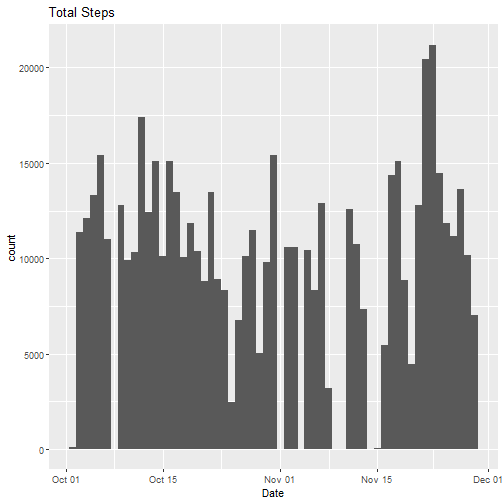
\includegraphics{stats-inf_files/figure-latex/unnamed-chunk-2-1.pdf}

Note that the histogram of the sample mean of the simulated data is
plotted along with the theoretical mean.\\
The red line indicates the theoretical mean and the black line is the
mean of the simulated data.\\
This figure clearly shows that the distribution of the simulated data is
centered around the theoretical mean. The difference between the sample
mean and the theoretical mean is \textbf{0.0049385}, which is fairly
small.

\hypertarget{sample-variance-versus-theoretical-variance}{%
\subsection{Sample Variance versus Theoretical
Variance}\label{sample-variance-versus-theoretical-variance}}

\begin{Shaded}
\begin{Highlighting}[]
\NormalTok{g =}\StringTok{ }\KeywordTok{ggplot}\NormalTok{(s,}\KeywordTok{aes}\NormalTok{(s))}
\NormalTok{sd_est =}\StringTok{ }\KeywordTok{mean}\NormalTok{(s}\OperatorTok{$}\NormalTok{s)}
\NormalTok{diff2 =}\StringTok{ }\KeywordTok{abs}\NormalTok{(sd_est}\DecValTok{-5}\NormalTok{)}
\NormalTok{g }\OperatorTok{+}\StringTok{ }\KeywordTok{geom_histogram}\NormalTok{(}\DataTypeTok{binwidth =} \FloatTok{0.3}\NormalTok{,}\DataTypeTok{color =} \StringTok{"black"}\NormalTok{,}\DataTypeTok{fill =} \StringTok{"red"}\NormalTok{) }\OperatorTok{+}\StringTok{ }\KeywordTok{geom_vline}\NormalTok{(}\DataTypeTok{xintercept =} \DecValTok{5}\NormalTok{,}\DataTypeTok{color =} \StringTok{"blue"}\NormalTok{,}\DataTypeTok{size =} \DecValTok{1}\NormalTok{) }\OperatorTok{+}\StringTok{ }\KeywordTok{geom_vline}\NormalTok{(}\DataTypeTok{xintercept =} \KeywordTok{mean}\NormalTok{(s}\OperatorTok{$}\NormalTok{s),}\DataTypeTok{size =} \DecValTok{1}\NormalTok{)}\OperatorTok{+}\KeywordTok{labs}\NormalTok{(}\DataTypeTok{title =} \StringTok{"Distribution of sample standard deviation"}\NormalTok{)}
\end{Highlighting}
\end{Shaded}

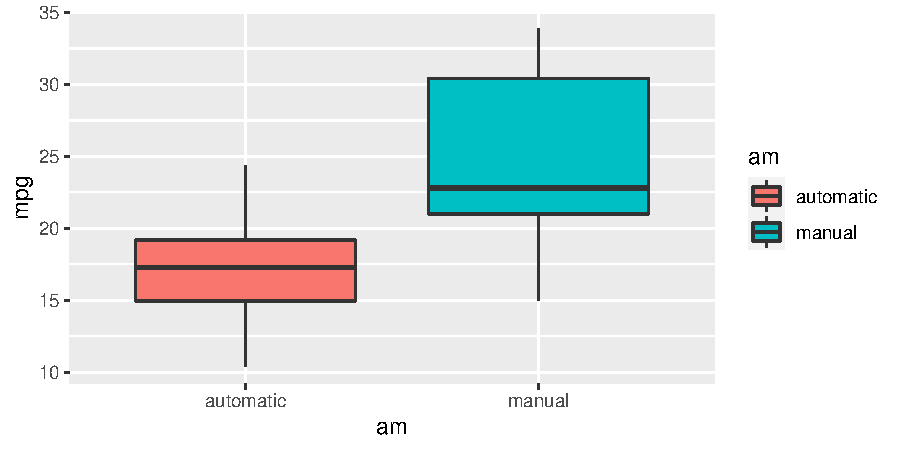
\includegraphics{stats-inf_files/figure-latex/unnamed-chunk-3-1.pdf}

Note that the histogram of the sample standard deviation of the
simulated data is plotted along with the theoretical standard
deviation.\\
The blue line indicates the theoretical standard deviation and the black
line is the standard deviation of the simulated data.\\
This figure clearly shows that the distribution of the simulated data is
centered around the theoretical standard deviation. The difference
between the sample standard deviation and the theoretical standard
deviation is \emph{0.0938222} and thus the difference between their
variances is the square of it which is \textbf{0.9294196}, which is
fairly small.

\#\#Distribution

\begin{Shaded}
\begin{Highlighting}[]
\NormalTok{x_sn =}\StringTok{ }\NormalTok{(x_bars}\OperatorTok{-}\NormalTok{mu_est)}\OperatorTok{/}\KeywordTok{sd}\NormalTok{(x_bars}\OperatorTok{$}\NormalTok{x_bars)}
\NormalTok{g =}\StringTok{ }\KeywordTok{ggplot}\NormalTok{(x_sn,}\KeywordTok{aes}\NormalTok{(}\DataTypeTok{x =}\NormalTok{ x_bars))}
\NormalTok{g}\OperatorTok{+}\KeywordTok{geom_histogram}\NormalTok{(}\KeywordTok{aes}\NormalTok{(}\DataTypeTok{y =}\NormalTok{ ..density..),}\DataTypeTok{binwidth =} \FloatTok{0.3}\NormalTok{,}\DataTypeTok{color =} \StringTok{"black"}\NormalTok{,}\DataTypeTok{fill =} \StringTok{"blue"}\NormalTok{)}\OperatorTok{+}\KeywordTok{stat_function}\NormalTok{(}\DataTypeTok{fun =}\NormalTok{ dnorm,}\DataTypeTok{args =} \KeywordTok{list}\NormalTok{(}\DataTypeTok{mean =} \KeywordTok{mean}\NormalTok{(x_sn}\OperatorTok{$}\NormalTok{x_bars),}\DataTypeTok{sd =} \KeywordTok{sd}\NormalTok{(x_sn}\OperatorTok{$}\NormalTok{x_bars)),}\DataTypeTok{size =} \DecValTok{2}\NormalTok{)}\OperatorTok{+}\KeywordTok{labs}\NormalTok{(}\DataTypeTok{title =} \StringTok{"Sample mean distribution and normal distribution"}\NormalTok{)}
\end{Highlighting}
\end{Shaded}

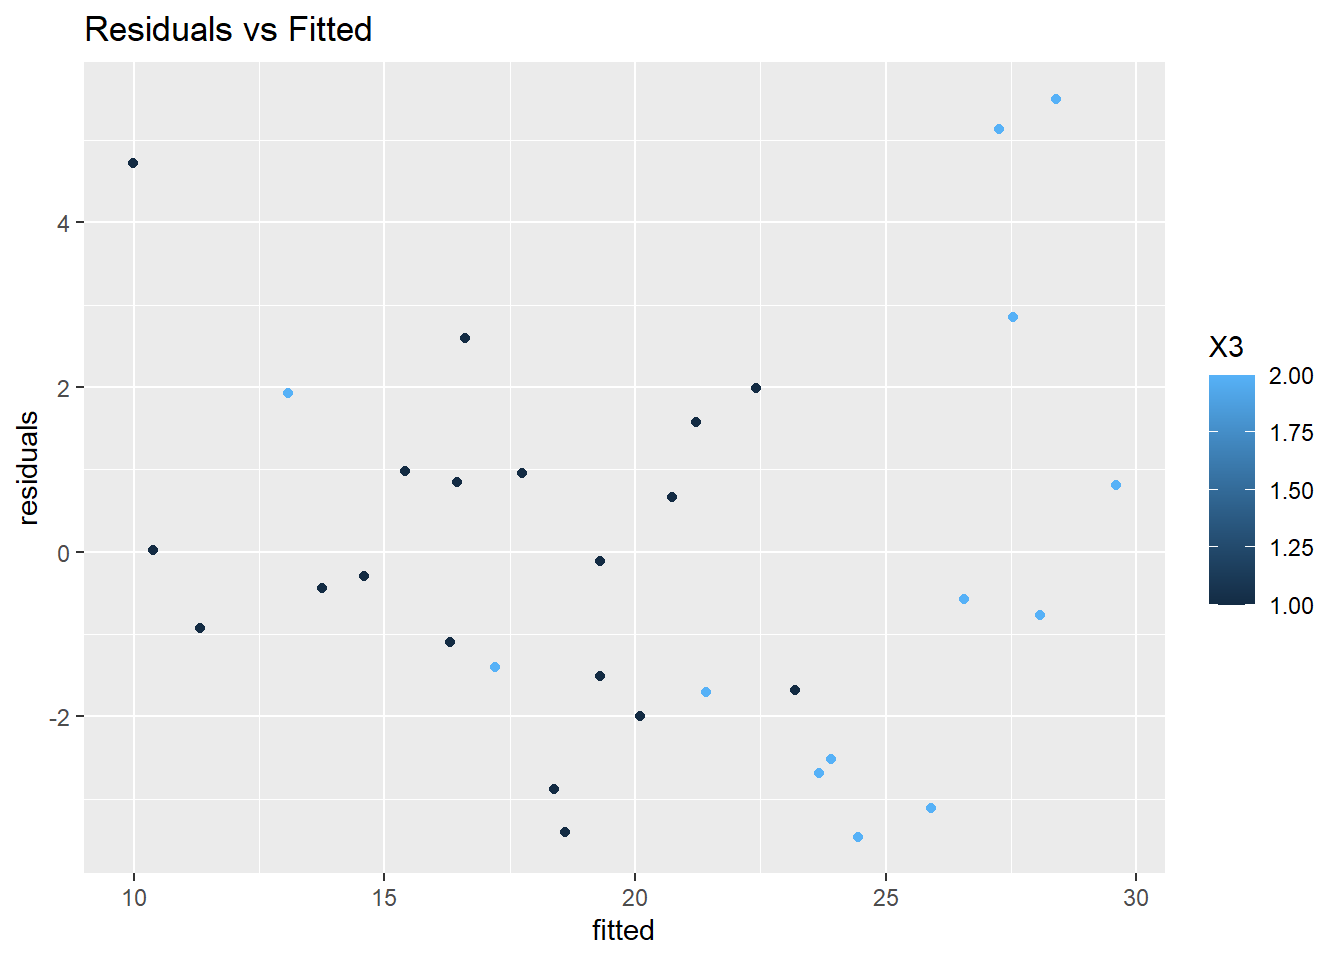
\includegraphics{stats-inf_files/figure-latex/unnamed-chunk-4-1.pdf}

This plot shows that the sample mean distribution is approximately equal
to the normal distribution.\\
As the normal distribution almost overlays the sample mean plot.

\end{document}
